\newpage

\section{Midterm 1 Review Problems}

\begin{prob}
Describe Euclid's construction for an equilateral triangle, and explain
why it works.
\end{prob}

\begin{prob}
Use the picture below to show that a pair of medians intersects at a point 2/3 of the way from the vertex to the opposite side.  Then use that fact to argue that the three medians must be concurrent.  
$$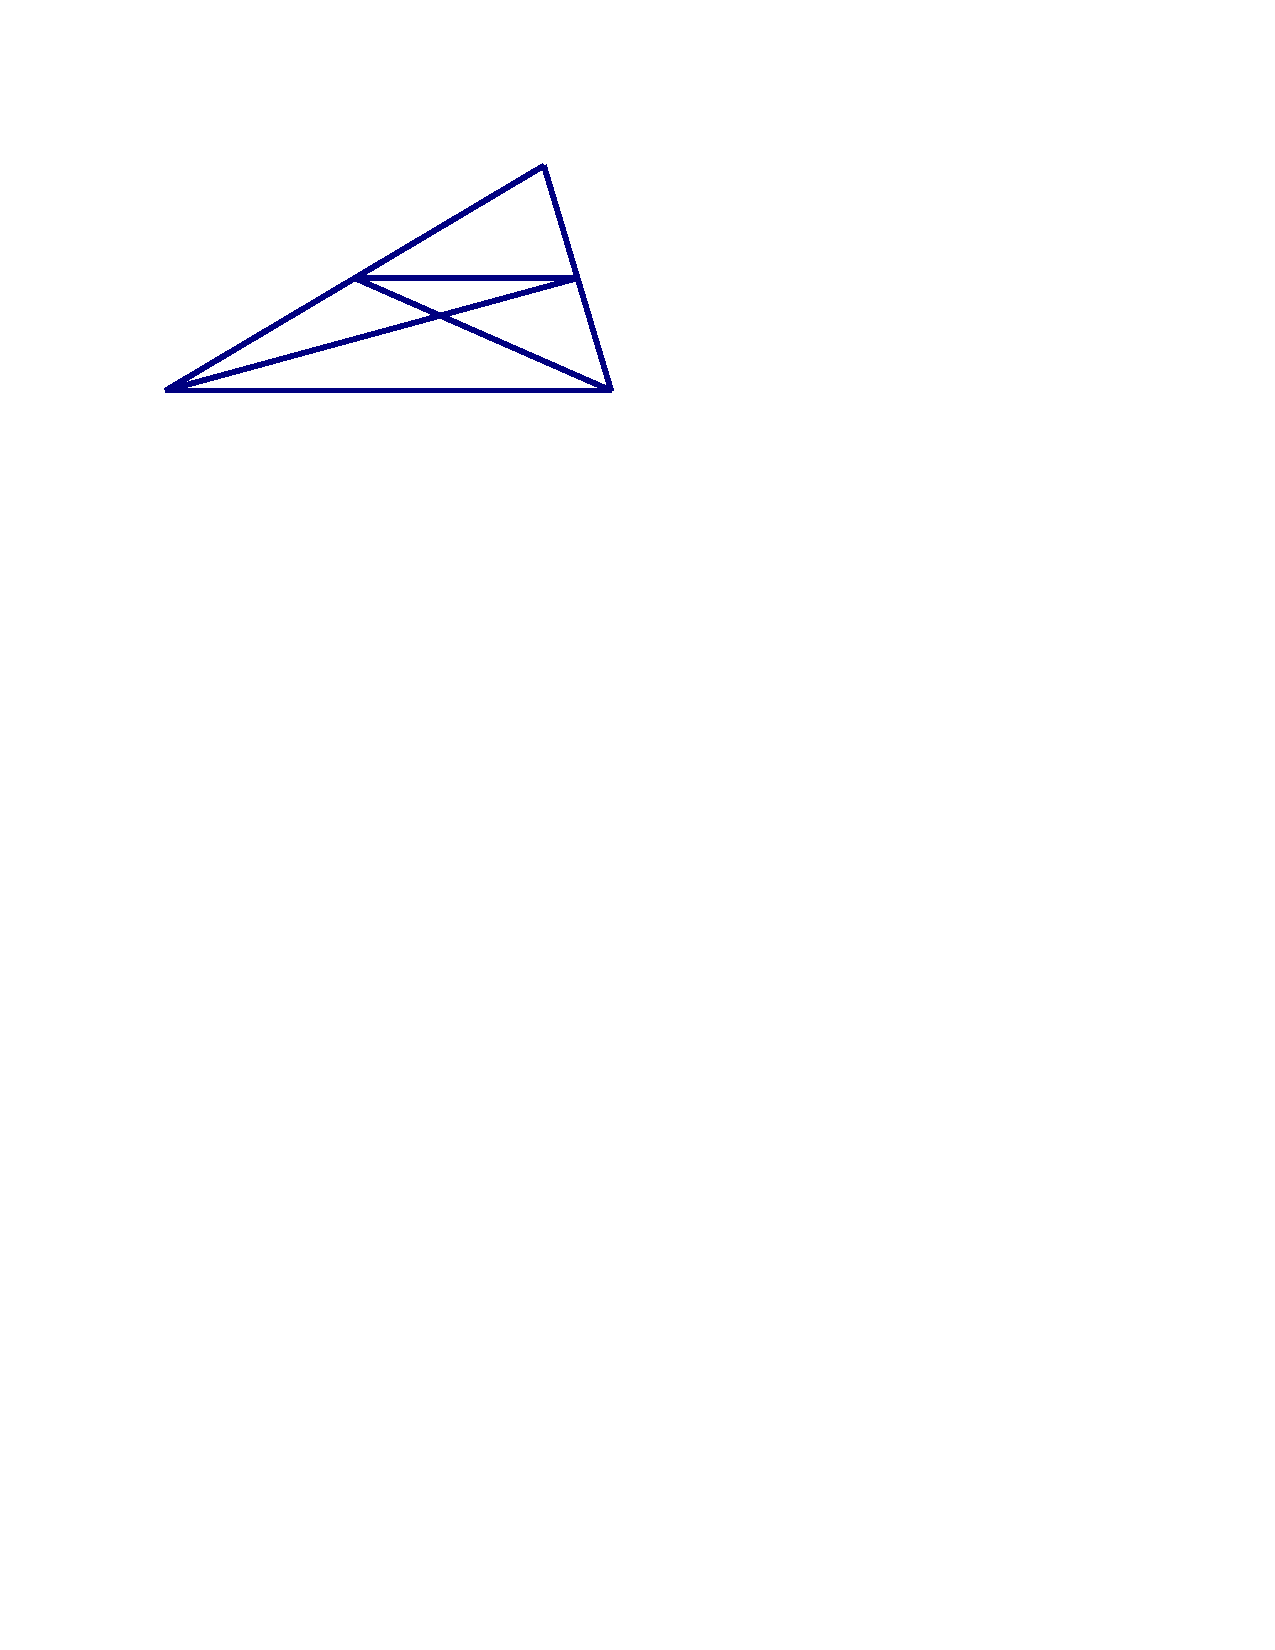
\includegraphics[width=2.5in]{../graphics/median1.pdf}$$
\end{prob}

\begin{prob}
Prove that the points on an angle bisector are \emph{exactly those} that are equidistant from the sides of the angle. 
\end{prob}

\begin{prob}
Show that, given any three non-collinear points in the Euclidean plane, there is a unique circle passing through the three points.
\end{prob}

\begin{prob}
Given a circle, give a construction that finds its center.
\end{prob}

\begin{prob}
State and prove a condition on any quadrilateral that is inscribed in a circle.  
\end{prob}

\begin{prob}
Construct a tangent line from a point outside a given circle to the circle.
\end{prob}

\begin{prob}
Give an informal derivation of the relationship between the circumference and area of a circle. 
\end{prob}

\begin{prob}
Prove:  If a quadrilateral is a parallelogram, then opposite sides are congruent.
\end{prob}

\begin{prob}
Prove:  If opposite sides of a quadrilateral are congruent, then it is a parallelogram.
\end{prob}


